\chapter{Formal model}
\label{chap:model}
We now aim to show how the consistency and dissemination of encounters can be ensured. 
For that purpose we define a model for interactions and their dissemination in a network of agents 
which resembles the TrustChain system. We also define a
mechanism to record information exchanges which allows to protect the network against free-riders who 
do not acquire and disseminate interaction records. Our proposal is to introduce \textit{exchange transparency} which can 
effectively punish free-riders. We further 
show that it is possible to detect agents that consciously interact with malicious agents, exposing
them as verification free-riders or accomplices.

\section{Model definition}
\label{sec:definitions}
We make use of the ordered interaction model which has been introduced in previous work by Otte et 
al.\ \cite{OTTE2017}. We restate it in Definition \ref{def:old_base} for clarity.
The symbols were annotated in order to reuse symbols in later definitions.

\begin{defn}[Ordered interaction model]. 
    \label{def:old_base}
    An ordered interaction model $\hat M = \langle \hat P, \hat I, \hat a, \hat w \rangle$ consists of two sets and two 
    functions.
    \begin{itemize}
        \item $\hat P$, a finite set of agents
        \item $\hat I$, a finite set of interactions
        \item $\hat a : I \rightarrow P \times P$, a function mapping each interaction to the agents 
        involved in it.
        \item $\hat w : I \times P \rightarrow \mathbb{R}_{\geq0}$, a function which describes the 
        contribution of an agent in an interaction
    \end{itemize}
\end{defn}

The model allows for the analysis of any type of application in which a network of agents performs
transactions that can be described by a quantitative amount. A more hands-on application of this 
model is Tribler. Similar to our description in Section \ref{sec:tribler}, agents model Tribler
instances, interactions are data transactions on the BitTorrent network where $w$ describes the 
net amount of data uploaded or downloaded. Also, interactions can in practice be recorded by 
TrustChain blocks which store the involved agents $a(i)$ and the amount of data $w(i)$.

However, the model does not explicitly
model the information exchange between agents. Our goal is to show that in a distributed trust system this 
exchange of information is also an essential component to guarantee manipulation resistance. We 
therefore extend the model with exchanges.

\begin{defn}[Ordered encounter model]
    \label{def:base}
    An ordered encounter model $M = \langle P, I, E, a, w, x \rangle$ is a 6-tuple consisting
     of three sets and three functions. For convenience we define a set $N = I \cup E$ as the set of all encounters.
    \begin{itemize}
        \item $P$, a finite set of agents
        \item $I$, a finite set of interactions
        \item $E$, a finite set of exchanges
        \item $a : N \rightarrow P \times P$, a function mapping each interaction and exchange to the agents 
        involved in it.
        \item $w : I \times P \rightarrow \mathbb{R}_{\geq0}$, a function which describes the 
        contribution of an agent in an interaction
        \item $x : E \times P \rightarrow \mathcal{P}(N)$, a function which describes the set of encounters that an 
        agent learns about in an exchange. $\mathcal{P}(N)$ denotes the power set of $N$.
    \end{itemize}
\end{defn}

Note that for any interaction $n \in I$ in which $p \notin a(n)$, $w(i,p) = 0$ must hold and similarly for any
exchange $e \in E$, $x(e, p) = \emptyset$ if $p \notin a(e)$.

An encounter $n \in N$ happens between two agents for one of
two reasons: to perform a transaction of some value or to exchange information.
The function $x$ describes a set of encounters that an agent obtains knowledge about through an 
exchange. A gossip protocol, that is the exchange of information with a random peer, is one way to create 
such exchanges. We will formally introduce the knowledge concept in Definition~\ref{def:subjective_network_state}.

For each agent we can describe the set of encounters that agent was involved in as the agent 
encounter history. 

\begin{defn}[Agent encounter history]
    Given an ordered encounter model $M = \langle P, I, E, a, w, x \rangle$ with encounters $N$ the 
    agent encounter history of an agent $p \in P$ is defined as follows:
    \begin{equation}
        H_p = \{ n \in N : p \in a(n) \}
    \end{equation}
    In a similar way the set of the agents interactions $I_p$ and $E_p$ can be defined.
    \begin{equation}
        I_p = \{ n \in I : p \in a(n) \}
    \end{equation}
    \begin{equation}
        E_p = \{ n \in E : p \in a(n) \}
    \end{equation}
\end{defn}

The history of any \textit{honest} agent $p$ is totally ordered by $<$. If we denote the 
$i$-th encounter of $p$ as $n_p(i)$ then we can alternatively write the agents history of length $t$ 
encounters as $H_p(t) = \{ n_p(1), n_p(2), ..., n_p(t)\}$. Similarly we can define $I_p(t)$ and 
$E_p(t)$ as the interactions and exchanges of $p$ after $t$ encounters. Note that $N_p(t) = I_p(t) \cap E_p(t)$. 
A \textit{dishonest} agent can break the order of their history. We will define this behavior in 
Definition \ref{def:double_spend}.

In our model encounters between agents are not public. This creates a discrepancy between the set of all
encounters $N$ and the known encounters from an agent $p$'s point of view. Agents only have 
knowledge of those encounters which they were involved in or which they obtained knowledge of through an exchange.
We can then define the subjective network state, which is the knowledge an agent has about the state of
the network.

\begin{defn}[Subjective network state]
    \label{def:subjective_network_state}
    Given an ordered encounter model $M = \langle P, I, E, a, w, x \rangle$  and an agent $p \in P$ 
    with encounter history $H_p$, the subjective network state of agent $p$
    is defined as follows:
    \begin{equation}
        N_p = H_p \cup \{ x(n, p) : n \in E_p \}
    \end{equation}
\end{defn}

Again we can denote the subjective network state of $p$ after $t$ encounters as $N_p(t)$.
The subjective network state contains the complete knowledge of the agent. Otte et al. define a
similar concept in the form of the subjective work graph. It generally models a partial view
of the network described by the model. This subjective view is the basis for their calculation of 
reputation and trust. The relation to the creation of trust is further discussed in Section \ref{sec:relevance}.

Agents can only reason about their subjective network state. Therefore an agent $p$ can only \textit{evaluate}
the function $x(e, q)$ if $e \subset N_p$ and $x(e,q) \subset N_p$.

The model from Definition \ref{def:base} introduces exchanges. Yet it does not define
how agents should exchange data. We therefore define an exchange policy. Any honest agent 
exchanges encounter information according to a given exchange policy.

\begin{defn}[Exchange policy]
    % Given an ordered encounter model $M = \langle P, I, E, a, w, x \rangle$
    % any exchange policy is a function $f : P \times I \rightarrow P \times \mathcal{P}(N)$.
    % An exchange policy defines for any interaction which information the involved agents
    % need to obtain from their partner in an exchange prior to the interaction. 
    An exchange policy is a function $f: P \times P \times \mathbb{Z} \times \mathbb{Z} \rightarrow \mathcal{P}(N) \times \mathcal{P}(N)$.
    For two agents $p$ and $q$ with histories $H_p(i)$ and $H_q(j)$ who would like to interact, 
    an exchange policy $f$ defines the sets $N^p \subseteq N_p(i)$ and $N^q \subseteq N_q(i)$ that 
    have to be sent by $p$ and $q$, respectively. We write $f(p,q,i,j) = (N^p, N^q)$.
\end{defn}

Our goal is to ensure that any honest agent adheres to the exchange policy defined for the network.
This will allow us to ensure that interactions are well disseminated and that agents cannot free-ride
on storing information.

% In order to check if an agent adheres to a certain exchange policy we need to know which 
% encounters an agent actually received in exchanges. So we can build a set $\epsilon_p$ in a similar
% way as the policy is defined. $\epsilon_p$ is a set of tuples where each tuple describes and 
% exchange $e$ with an agent $q$ in which encounters $x(e, p)$ were received from which agent: 

% \[ \epsilon_p := \{ (q, x(e, p)) : e \in H_p \cap E,  \exists (p, q) \in a(e)\}\]

As the exchanges are part of an agents history it is possible to determine whether an agent has always
exchanged in accordance with a certain exchange policy. 

\begin{defn}[Exchange policy adherence]
    \label{def:adherence}
    Given an agent $p$, $p$ adheres to the policy $f$ if for every interaction $n(k) \in I_p$ with
    partner agent $q$ there exists a unique exchange $n(i) \in E_p(k-1)$ such that 
    $N^q \subseteq x(p, n(i))$ and $N^p \subseteq x(q, n(i))$, where $N^q$ and $N^p$ are defined 
    through $f(p,q,i-1,j-1)=(N^q, N^p)$.
\end{defn}



% We can define an algorithm that determines whether an agent 

% \begin{algorithm}
% \caption{Exchange verification}\label{alg:verify_exchange}
% \begin{algorithmic}[1]
% \Procedure{verifyPolicyAdherence}{}
% \State {$f$ \leftarrow Exchange policy to be verified}
% \ForAll{interactions $n(i)$ in $I_p(t)$}
% \State {$(\_,q) \leftarrow a(n(i))$}
% \If {$\not\exists e(j) \in E_p(i)$ such that $a(e(j)) = (p,q)$, $j < i$ and $e(j)$ is not marked}
% \Return {false}
% \EndIf
% \State {mark $e(j)$}
% \State {$N^p \leftarrow$ data that p needs to send according to $f$}
% \State {$N^q \leftarrow$ data that q needs to send according to $f$}
% \If {$N^q \nsubseteq x(p,e(j))$ or $N^p \nsubseteq x(q,e(j))$}
% \Return {false}
% \EndIf
% \EndFor
% \Return true
% \EndProcedure
% \end{algorithmic}
% \end{algorithm}

% The subjective network state also implies the known agents $P_p = \{ q \in P : n \in N_p, q \in a(n) \}$
% Without full observability there is also no guarantee that agents know the full history of their 
% peers. Actually the subjective network state defines also $p$'s observed peer history of an agent $q$.

% \begin{equation}
%     H_{p, q} = \{ n \in N_p : q \in a(n) \}
% \end{equation}

% Similar the observed peer history is a totally ordered set. It is not necessarily equal to the 
% complete history though. For example, an agent $q$'s history $H_{q} = \{n_q(1), n_q(2), n_q(3) \}$
% could be observed by an agent $p$ as $H_{p, q} = \{n_q(1), n_q(3)\}$.

% Finally, a reputation mechanism needs to be defined. Agents estimate the reputation of their peers
% from their subjective network state. 

% \begin{defn}[Reputation mechanism] 
%     A reputation function $R$ takes as input the subjective network state $N_{p}$ and determines 
%     a reputation score $S^R_{p,q}(I_{p,q}) \in \mathbb{R}$ for all known agents $P_p$.
% \end{defn}

\section{Fork and double spend defense}
\label{sec:model_double_spend}
In what follows we analyze the defense of certain exchange policies against a double spend attack. 
That attack is a potent attack on a network that can be modelled by an ordered encounter model. 
Conceptually, an attacker 
has two conflicting interactions at the same time with two different agents. Each partner is not
aware of the other, therefore both accept the interaction. 

\begin{defn}[Fork and double spend]
    \label{def:double_spend}
    Given an ordered encounter model $M = \langle P, I, E, a, w, x \rangle$, a malicious agent $p$ has two conflicting interactions 
    $i \in I$ and $j \in I$ at the exact same time such that $i = n_p(t)$ and $j = n_p(t)'$. Both interactions have a different partner $a(i) = (p, q)$ 
    and $a(j) = (p, r)$. Accordingly, the history  of $p$ is not a totally ordered set anymore.
    The attack can be detected if for any honest agent $s$, $i \in N_{s}$ and $j \in N_{s}$ are
    true.
\end{defn}

In the following we show that exchanging blocks is essential for the network to defend against such an 
attack. We first study the case of no exchanges. For that we formally define the No-Exchange policy.

\begin{pol}[No-Exchange]
    \label{pol:no-exchange}
    The No-Exchange policy $f^{\text{NE}}$ defines no required exchanges for an honest agent, so for 
    any two agents $p$ and $q$ and any lengths of their encounter histories $i$ and $j$, 
     $f^{\text{NE}}(p,q,i,j) := (\emptyset, \emptyset)$.
\end{pol}

Without any exchanges, agent are only aware of the interactions that they perform themselves. In
Figure \ref{fig:no_exchange_policy} we visualize a situation in which five honest agents perform interactions. 
The timeline of each agent is represented by the horizontally dashed line. Each interaction is 
connected to two agents' timelines. The No-Exchange policy requires no information exchange so agents only have
interactions. Each connected interaction is part of an agent's history. The figure indicates with 
blue, the blocks that agent F is aware of which are only those he was involved in.

\begin{figure}
    \centering
    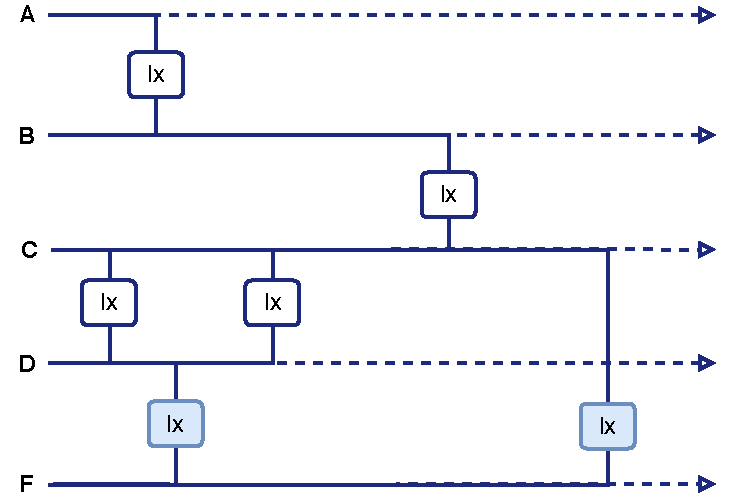
\includegraphics[width=0.5\textwidth]{images/no_exchange_policy.pdf}
    \caption{History graph of a network  No-Exchange policy in our model. We consider 5 agents. Each agent has a time
    line which is connected to interactions(denoted by Ix). Each interaction is between two agents. 
    The blue blocks show the subjective network state of agent F.}
    \label{fig:no_exchange_policy}
\end{figure}

\begin{thm}[Detectability of double spend without exchanges]
    \label{thm:fork_no_gossiping}
    If honest agents apply the No-Exchange policy, the fork and double spend attack cannot be detected by any honest agent.
\end{thm}
\begin{proof}
    Let $p$ be the attacking agent and let $i$ and $j$ be the conflicting interactions of the 
    attacks. Further, let $q$ be the partner in interactions $i$ such that $a(i) = (p, q)$ and let 
    $r$ be the partner of interaction $j$ such that $a(j) = (p, r)$. 
    The No-Exchange policy implies that for any honest agent $s \in P$ and all $e \in E$, $x(e, s) = \emptyset$ 
    and therefore $N_s = H_s$ applies. 
    According to Definition \ref{def:subjective_network_state} $i \in N_{q}, j \notin N_{q}$ and 
    $i \notin N_{r}, j \in N_{r}$. 
    Furthermore, for any honest $s \in P$, $i \notin N_s$ and $j \notin N_s$ must be true because
    $s \notin a(i)$ and $s \notin a(j)$.
    % Without gossiping both $q$ and $r$ will not further disseminate 
    % their interactions with $p$ and therefore will not learn of the other version.
    % Moreover, all other agents $s \in P$ are aware of neither $i$ or $j$ because only direct 
    % interactions are observed. Consequently no agent observes both $i$ and $j$.
\end{proof}

Theorem \ref{thm:fork_no_gossiping} proves that the double spend attack cannot be
detected without exchanging encounters. 

We now show that if agents do exchange information, this can lead to the detection of the attacker. We
define an exchange policy in which honest agents obtain the encounter history prior to an interaction.

\begin{pol}[History-Exchange policy]
    \label{pol:one}
    The History-Exchange policy $f^{\text{HE}}$ requires for 
    any two agents $p$ and $q$ and any lengths of their encounter histories $i$ and $j$: 

    \begin{equation}
        f^{\text{NE}}(p,q,i,j) := (H_p(i), H_q(j))
    \end{equation}
\end{pol}

Figure \ref{fig:chain_exchange} shows the same 5 agents, with the same interactions. This time agents
apply the History-Exchange policy, which requires the exchange of both agents' histories prior to 
an interaction. The colored interactions and exchanges are received by F, green being those received
from D and purple those received from C. At the end of the shown timeline, the colored blocks are 
the subjective network state of F.

\begin{figure}
    \centering
    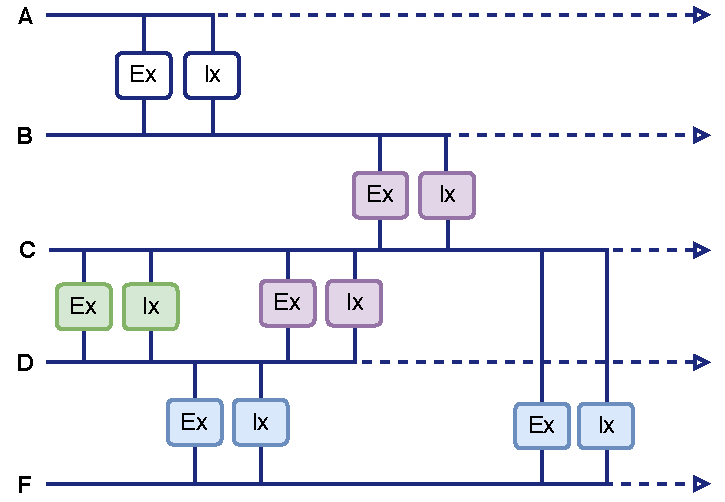
\includegraphics[width=0.5\textwidth]{images/chain_exchange.pdf}
    \caption{History graph of History-Exchange policy in our model. We again consider 5 agents. The 
    colored blocks show the subjective network state of agent F. The blue blocks are F's own encounters,
    the green block is an encounter received from D while the purple blocks are received from C.}
    \label{fig:chain_exchange}
\end{figure}

\begin{thm}[Detectability of double spend with the History-Exchange policy]
    \label{thm:fork_gossiping}
    If all honest agents apply the History-Exchange policy and periodically use uniform sampling over
    the set of agents to find an interaction partner, the double spending will eventually be detected.
\end{thm}
\begin{proof}
    Let $p$ be a malicious agent, with $H_p(t-1)$ and let $n(t) \in I$ and $n(t)' \in I$ be the conflicting 
    interactions of the attack. 
    Further, let $q$ be the partner in interaction $n(t)$ such that 
    $a(n(t)) = (p, q)$ and let $r$ be the partner of interaction $n(t)'$ such that $a(n(t)') = (p, r)$. 
    According to Definition \ref{def:subjective_network_state} $i \in N_{q}, j \notin N_{q}$ and 
    $i \notin N_{r}, j \in N_{r}$.

    We consider an honest agent $q$ sampling agents for an interaction after the double spend. 
    For network size $l = |P|$ the 
    probability of choosing partner $r$ in the first round is $1/l$. The probability for not having
    chosen $r$ in any of $k$ rounds is $(\frac{l-1}{l})^k$ and $\lim_{k\to\infty}(\frac{l-1}{l})^k = 0$.
    Given an infinite amount of time, $q$ therefore chooses $r$ for an interaction $k$ and because $q$ is 
    honest they do an exchange $e$ prior to their interaction. 
    
    Before the exchange, $j \in H_r$ holds. Both $r$ and $q$ are honest and adhere to the exchange 
    policy $f^{\text{HE}}$, therefore $j \in x(e, q)$ holds. This means that after the exchange $e$, 
    $i \in N_q \text{ and } j \in N_q$ holds. Therefore $q$ is able to detect the double spending.
\end{proof}

Theorem \ref{thm:fork_gossiping} shows that exchanging encounter information makes double spending detectable. Once a double
spender is detected by an agent it is possible to ignore them for future interactions. The amount 
of exchange rounds until the detection depends on the exact policy of exchanging data and a deeper 
analysis is beyond the scope of this work. However, qualitatively, exchanging more information in
each exchange obviously leads to faster detection.

\section{Exchange free-riding}
We now look at ways to incentivize information exchanges. At this point we have shown that in a network in which 
interactions are only directly observable by the involved agents, an exchange mechanism like the
History-Exchange policy is essential to defend against the double-spending attack. 
Our aim is now to show that such an exchange policy can be ensured. Conceptually, if the exchange 
behavior is visible in the history of an agent, any missing or incomplete exchange will uncover 
that agent as a fraud.

We consider an incentive not to exchange encounter information.
If bandwidth and storage capacity are valuable resources for agents, data dissemination and their 
long-term storage come at a cost for agents. Therefore agents can attempt to be lazy and only 
interact without exchanging the necessary data. 
However if all agents would behave in that way the system loses 
the ability to defend itself against forks and double spending as shown in Theorem 
\ref{thm:fork_no_gossiping}. We will call those lazy agents \textit{exchange free-riders}. 

% An honest agent should also be able to verify that other agents adhere to an exchange policy or not.

% \begin{lem}[Exchange policy adherence]
%     \label{lem:policy_adherence}
%     Given an ordered encounter model $M$ with exchange policy $D$, any agent $p$ that has observed 
%     the complete history $H_s$ of an agent $s$ can determine whether that agent adhered to policy 
%     $D$.
% \end{lem}
% \begin{proof}
%     Agent $p$ has observed the complete history of agent $q$, therefore $H_q \subseteq N_p$. Agent 
%     $p$ is then able to calculate the frequency of $q$'s exchanges as $f^D_q = \frac{|\{ n \in H_q : n \in E \}|}{|\{ n \in H_q : n \in I \}|}$,
%     the partners of exchanges $S^D_q = \{ a(n) \setminus q : n \in H_q \text{and} n \in E \}$ and the 
%     exchanged encounter $E^D_q = \{ x(n,q) : n \in H_q \text{and} n \in E \}$. Then $p$ can compare
%     the calculated values to the expected values defined by $D$. 
% \end{proof}

\begin{defn}[Exchange free-rider]
    \label{def:gos_free-rider}
    Given an exchange policy $f$ that all honest agents use, an exchange free-rider is a dishonest 
    agent $p$ whose encounter history $H_p$ does not adhere to policy $f$ as defined by Definition \ref{def:adherence}.
    % Given an ordered encounter model $M = \langle P, I, E, a, w, x \rangle$ with exchange policy $f$, an exchange free-rider $p \in P$ is an 
    % agent whose exchange behavior does not fulfill the minimum requirements of policy $f$. That is, 
    % $f(I_p) \nsubset \{ (q, x(e, p)) : e \in H_p \cap E, \exists (p, q) \in a(e)\}$.
\end{defn}

Any failure to send or receive the correct encounter information before an interaction will make 
an agent an exchange free-rider.
We now show that any honest agents will not commit to an interaction with an exchange free-rider

\begin{thm}[No interaction without correct exchange]
    \label{thm:no_interaction}
    An honest agent who adheres to the History-Exchange policy can not interact without a successful 
    exchange except with a double-spender.
\end{thm}
\begin{proof}
    Given the History-Exchange policy $f^{\text{HE}}$, an honest agent $p$ with encounter history $H_p(i)$ and a potential 
    partner $q$ with history $H_q(j)$, $p$ will request an exchange $e$, such 
    that $e = n_p(i+1) = n_q(j+1)$ in order to be in accordance with $f^{\text{HE}}$. 
    $f^{\text{HE}}$ further defines that $p$ needs to send $H_p(i)$ and $q$ needs to send $H_q(j)$.
    Also, because $p$ is honest, $p$ will send the correct data such that $H_p(t_p) \subseteq x(q,e)$. 
    
    The correctness of the exchange depends on the behavior of $q$.
    Only if $q$ also sends the correct information such that $H_q(t) \subseteq x(p,e)$, do $p$ and $q$ comply with 
    the exchange policy $f^{\text{HE}}$. 
    
    $p$ can verify whether $H_q(t_q) \not\subset x(p,e)$ if there exists some $k$, $1 \leq k \leq j \in \mathbb{Z}, n_q(k) \notin x(p,e)$. If 
    $p$ finds that $H_p(t_p) \subseteq x(q,e)$, $p$ can conclude that either $q$ has sent the correct
    encounters, or $q$ is attempting a fork if there exists $n_q(t_q+1) \notin x(q,e)$.
    
    In order to not create proof of being an exchange free-rider, $p$ cannot interact with $q$ if 
    $p$ finds the exchange to be incomplete.
\end{proof}

% \begin{thm}[Detectability of exchange free-riders]
%     \label{thm:gos_free-rider}
%     Given an ordered encounter model $M = \langle P, I, E, a, w, x \rangle$ in which honest agents use the 
%     History-Exchange policy an exchange free-rider will be detected on the first interaction.
% \end{thm}
% \begin{proof}
%     Assume agent $p$ is an honest agent and is about to interact with agent $q$. Because agent $p$
%     uses Policy \ref{pol:one}, $p$ will request an exchange with $q$. That exchange will contain 
%     $H_q$. If it does not $p$ will know that $q$ is a exchange free-rider. After a successful
%     exchange $H_q \subseteq N_p$. In that case $p$ is able to build the set of received blocks for 
%     each exchange defined by $\epsilon_q := \{ (r, x(e, q)) : e \in H_q \cap E,  \exists (q, r) \in a(e)\}$. Then $p$ check the condition for adherence to 
%     the History-Exchange policy $f$ by $f(I_q) \subseteq \epsilon_q$. If the condition is not true agent $p$ has found $q$ to be a
%     exchange free-rider.
% \end{proof}

According to Theorem \ref{thm:no_interaction} any honest agent who applies the history exchange policy
can ensure that no free-riding happens in their encounters except if their partner attempts to fork. 
Note that the architecture we present cannot prevent the creation of forks, however eventual fork
detection has been proven in Theorem \ref{thm:fork_gossiping}. Only with collusion two agents can 
attempt to not exchange the correct data and still interact.
Such historical free-riding with third-parties cannot be detected with the History-Exchange policy.
In the next section we define a policy that does allow this.

The incentive to not commit an interaction without a complete exchange is created through the 
recording of the exchange on the history of the agent. If an agents history proves an incomplete exchange 
before an interaction, the agent does not adhere to the exchange policy anymore according to 
Definition~\ref{def:adherence}. We show in the next section that if any agent has the complete subjective network state 
of another agent, the complete history of an agent can be verified to no include any free-riding 
on the exchanges.

\section{Verification free-riding}
\label{sec:verification_free-riding}
We have shown that forks will eventually be detected and that free-riding is not possible in an 
encounter with an honest agent. However, free-riding in other encounters cannot be detected and 
agents who do not perform or ignore consistency checks, and thus interact with double spender cannot
be detected. 


In order to solve those two problems, a stronger exchange policy can be enforced. This will allow 
to audit the complete history of another agent and detect any inconsistencies or incorrect behavior.

% We can define Algorithm \ref{alg:verify_exchange} which is run by all 
% honest agents for each exchange in order to defend against double-spenders and exchange free-riders.

% \begin{algorithm}
% \caption{Exchange verification}\label{alg:verify_exchange}
% \begin{algorithmic}[1]
% \Procedure{verifyExchange}{}
% \State {$p$: Honest agent, receiver of exchange}
% \State {$q$: Agent, subject of verification}
% \State {$H_q$ \leftarrow $q$'s encounter history}
% \State {$N_p$ \leftarrow $p$'s subjective network state}
% \ForAll{exchanges $e$ in $H_q$ }
% \If {$e$ is not valid according the the exchange policy} \Return false
% \EndIf
% \EndFor
% \ForAll{interaction $i$ in $H_q$}
% \If {$i$ is in conflict with any $j \in N_p$} \Return false
% \EndIf
% \EndFor
% \Return true
% \EndProcedure
% \end{algorithmic}
% \end{algorithm}

% Similar to exchanging data the execution of Algorithm \ref{alg:verify_exchange} introduces
% some costs for agents. Therefore agents again could try to manipulate the system by not verifying 
% the encounters and instead blindly accepting the received information. We will define those agents
% as verification free-riders.

% \begin{defn}[Verification free-riders]
%     A verification free-rider is an agent that does not verify received exchanges using Algorithm 
%     \ref{alg:verify_exchange}.
% \end{defn}

% In contrast to the detection of exchange free-riders, the detection of verification free-riders is
% less straight-forward because the execution of an algorithm is not directly observable. An honest agent
% that always verifies the encounters received from peers will not interact with double spenders or 
% exchange free-riders. A verification free-rider on the other hand cannot discern between honest,
% malicious and free-riding peers. Hence, should there be a malicious agent $q$ and a verification 
% free-rider $r$ chances are that $q$ and $r$ will interact. Should $r$ have the information to know 
% that $q$ was malicious and still interacted, then this behavior is different from an honest agent.
% We aim to detect this behavior in order to protect against verification free-riders.

In order to perform such a deep analysis, honest agents need to obtain the full subjective network 
view of another agent before each interaction. Therefore we define the Network-State-Exchange policy.

\begin{pol}[Network-State-Exchange]
    \label{pol:network_state}
    % The Network-State-Exchange policy requires agents to obtain the subjective network state of their partner 
    % prior to an interaction. 

    % \[ f(I_p) := \{ (q, N_q) : \exists i \in I_p, q \in a(i) \}\]
    The Network-State-Exchange policy $f^{\text{NSE}}$ requires for 
    any two agents $p$ and $q$ and any lengths of their encounter histories $i$ and $j$:

    \begin{equation}
        f^{\text{NSE}}(p,q,i,j) = (N_p(i), N_q(j))
    \end{equation}
\end{pol}

In order to visualize the difference to the other exchange policies, we show the same 5 agents in Figure \ref{fig:network_state_exchange}, 
with the same interactions. This time agents apply the Network-State-Exchange policy, which requires
the exchange of both agents' subjective network state prior to an interaction. In contrast to the 
History-Exchange policy, this time F also received knowledge about interactions from agents A and B.
The policy greatly increases the storage requirements. We will consider this in Section \ref{sec:storage}.

\begin{figure}
    \centering
    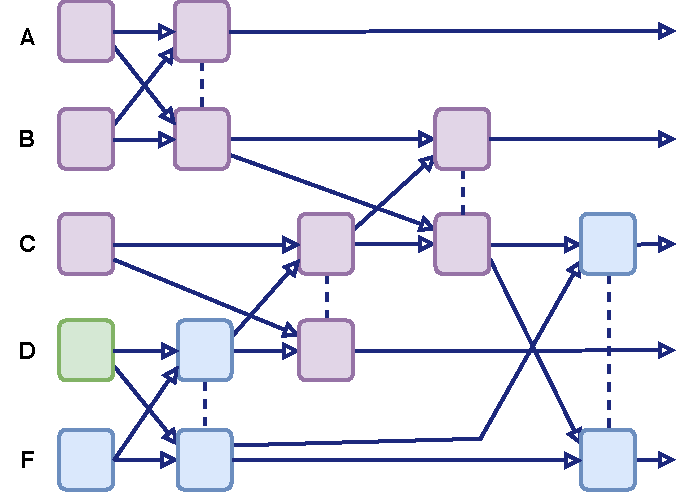
\includegraphics[width=0.5\textwidth]{images/network_state_exchange.pdf}
    \caption{History graph of Network-State-Exchange policy in our model. We again consider 5 agents. The 
    colored blocks show the subjective network state of agent F. The blue blocks are F's own encounters,
    the green block is an encounter received from D while the purple blocks are received from C. This
    time F obtains the complete network state.}
    \label{fig:network_state_exchange}
\end{figure}

% We can define a
% property 

% \begin{defn}[Subjective network state transparency]
%     Given is an ordered encounter model $M = \langle P, I, E, a, w, x \rangle$Let $p$ be an honest agent that applies the Network-State-Exchange policy and let $q$ be an agent
%     that exchanged with $p$. According to Policy \ref{pol:network_state} after a succesful exchange
%     $N_q \subset N_p$ and thus also $H_q \subset N_p$. As previously defined the agent encounter
%     history is a totally ordered set. Let $n_q(t)$ denote the $t$th encounter of agent $q$. At each
%     round $t$ the $q$'s subjective network state is given by $N_q(t) = \{ n \in N : n \in H_p(t-1) \} \cup \{ x(e, p) : e \in E \text{ and } e \in H_p(t-1) \}$.
% \end{defn}

We first show that if an agent $p$ knows the subjective network state, that is the full knowledge of 
another agent $q$, $p$ is able to determine whether $q$ adhered to the Network-State-Exchange policy.


\begin{lem}[Verification of adherence to policy]
    \label{lem:detection_free-rider}
    Given the subjective network state $N_q(t)$ of an agent $q$, an agent $p$ is able to 
    determine whether that agent adhered to the Network-State-Exchange policy.
\end{lem}
\begin{proof}
    For every interaction $n_q(i) \in I_q(t)$ with a partner $s \in P$ there should exist a 
    unique exchange $e$ such that $a(e) = (q,s)$ and $e = n_q(j) = n_s(k)$. If the exchange
    is correct $N_s(k-1) \subseteq x(e,q)$ and thus $N_s(k-1) \subset N_q(t)$. 
    
    If $p$ knows $N_q(t)$, $p$ can evaluate whether $N_s(k-1)$ is in $N_q(t)$ because $H_s(k-1)$ 
    must also be in $N_q(t)$.
    
    According to Definition \ref{def:subjective_network_state}, $N_s(k-1)$ can be inferred from the 
    history $H_s(k-1)$ by evaluating $x(n_s, s)$ for all exchanges $n_s \in E_s(k-1)$. 
    If $p$ for any $s$, $p$ cannot evaluate any $x(n_s, s)$, that means that some $n \in x(n_s, s)$ 
    is not in $N_q(t)$. In that case $q$ cannot be honest because $q$ can also not evaluate 
    $x(n_s, s)$.
\end{proof}

The previously defined lemma allows us to prove that any honest agent, in a network that applies the
Network-State-Exchange policy, can verify whether their partner has up to the point of their encounter
adhered to the policy.

\begin{thm}[Detectability of free-riding]
    \label{thm:ver_free-rider}
    An honest agent who applies the Network-State-Exchange policy is able to verify whether another
    agent is a free-rider.
\end{thm}
\begin{proof}
    Let $p$ be an honest agent who applies the Network-State-Exchange policy and let $q$ be an agent
    that exchanged encounters with $p$. Let $e$ be their latest exchange such that $e = n_p(i) = n_q(j)$
    and $N_q(j-1) \subset N_p(i)$ should hold.
    
    $p$ can ensure that $x(e, p) = N_q(j-1)$ because $N_q(j-1)$ includes $H_q(j-1)$ and $N_q(j-1)$
    can be inferred from $H_q$ by evaluating $x(n_q, q)$ for all exchanges $n_q \in E_q(j-1)$.
    If any $x(n_q, q)$ cannot be evaluated, this means that $N_q(j-1)$ is not complete.
    Otherwise it holds that $N_q(j-1) \subset N_p(i)$. 

    According to Lemma \ref{lem:detection_free-rider} $p$ is then able to verify whether 
    $q$ adhered to the Network-State-Exchange policy.
\end{proof}

This creates a stronger guarantee than Theorem \ref{thm:no_interaction} as even historic dishonest
behavior is detected and leads to that agent being ignored.

The Network-State-Exchange behavior further allows any agent $p$ that exchanged information with an agent $q$
to reconstruct the subjective network state of agent $q$ after any encounter $j$. 
This makes it possible for an honest agent $p$ to re-evaluate $q$'s decisions to engage in each of $q$'s 
interactions.

\begin{thm}[Detectability of interactions with double-spender]
    \label{thm:ver_free-rider}
    An honest agent who applies the Network-State-Exchange policy is able to detect any wrongful
    interaction with a double spender.
\end{thm}
\begin{proof}
    Let $p$ be an honest agent who applies the Network-State-Exchange policy and let $q$ be an agent
    that exchanged encounters with $p$. Let $e$ be their latest exchange such that $e = n_p(i) = n_q(j)$
    and because $p$ is honest, $x(e, p) = N_q(j-1)$ and $x(e,q) = N_p(j-1)$. 
    Therefore it holds that $N_q(j-1) \subset N_p(i)$. This implies also that any previous 
    subjective network state of $q$, so for any $1 \leq k \leq j-1$, $N_q(k) \subset N_p(i)$. Then,
    for all $k$, $p$ can determine the set of double-spender (malicious) $P^m(k)$ agents that $q$
    was aware of after $k$ encounters. If there exists an interaction $n_q(l)$ with some malicious
    agent $s$ and $l>k$, $p$ finds that $q$ knowingly interacted with a malicious agent or did not
    perform the verification to find $s$. Both cases are considered dishonest behavior.
\end{proof}

We have shown in Theorem \ref{thm:ver_free-rider} that the Network-State-Exchange policy enables 
agents to effectively find any wrongful interactions with double spenders. If $p$ finds $q$ to
be wrongful, $q$ either colluded with a double spender or $q$ did not find the double spender which 
means $q$ did not perform the right verifications. In the latter case we call $q$ a verification 
free-rider.

We can combine our findings in an audit algorithm which allows an honest agent $p$ to establish the 
correctness of another agent $q$'s encounter history. 

\begin{algorithm}
\caption{Audit algorithm which verifies that an agent has adhered to the Network-State-Exchange 
policy and has not knowingly interacted with a malicious agent}\label{alg:verify_exchange}
\begin{algorithmic}[1]
\Procedure{historyAudit}{$N_q(t)$}
\State {$P^v \leftarrow \emptyset$, set of valid next interaction partners}
\State {$P_m \leftarrow \emptyset$, set of detected malicious agents}
\State {$N_q(0) \leftarrow \emptyset$, $q$'s subjective network state}
\ForAll{encounters $n(i)$ in $N_q(t)$ }
\State {$s \leftarrow$ partner in $n(i)$ such that $a(n(i)) = (q, s)$}
\State {$N_q(i) \leftarrow N_q \cup \{n(i)\}$}
\If {$n(i)$ is an interaction} 
\If {$s$ is in $P^m$}
\State {\Return false}
\ElsIf {$s$ is not in $P^v$}
\State {\Return false}
\Else
\State {$P^v \leftarrow P^v \setminus \{s\}$}
\EndIf
\EndIf
\If {$n(i)$ is an exchange}
\State {$N_q(i) \leftarrow N_q(i) \cup x(n(i),q)$}
\If {$x(n(i),q) = N_s(j)$}
\State {$P^v \leftarrow P^v \cup \{s\}$}
\EndIf
\If {$\exists r \in P, n_r(t), n_r(t)' \in N_q(i)$}
\State {$P^m \leftarrow P^m \cup \{r\}$}
\EndIf
\EndIf
\EndFor
\Return true
\EndProcedure
\end{algorithmic}
\end{algorithm}

At this point the question arises who verifies that agents perform this detection of verification 
free-riders. The detection of verification free-riders is a recursive problem and therefore will not
lead to an infinite verification process. However, because agent exchange their complete subjective
network state, they also share their knowledge of malicious agents and free-riders. Suppose an agent
$p$ is aware of a set of malicious agents $S_p$. After exchanging all information with another agent
$q$, $q$'s set of malicious agents should at least contain $S_p \subseteq S_q$. Should an agent $q$ 
interact with any agent in $S_p$, at least agent $p$ knows that $q$ is dishonest. This way $q$ will 
slowly be isolated.

\section{Relevance for global trust system}
\label{sec:relevance}
The calculation of reputation and trust has not been part of the discussion up to now.
This brings about the question of relevance to the global trust system. We refer again to the work
of Otte et al. for an in depth study of interaction graph based trust mechanisms.
The authors show that scoring mechanisms based on a graph representation the interactions between 
agents can be designed to be resilient against Sybil-attacks. For their analysis the authors use the
model stated in Definition \ref{def:old_base} as the basis for creating a graph. 

The mechanisms described in this chapter improve trust systems by ensuring that the encounters which
are the basis of the calculations of trust and reputation are honest, well disseminated and consistent.
We mention in this section a few conclusions that we can draw from the above theoretical analysis.

\subsection{Manipulation resistance}
Instead of exploring new ways of calculating trust, we analyzed in the above the resilience to of 
the model in the presence of malicious and free riding agents. We have shown that in order to defend
against forks and double spending, information exchange between agents is critical. Only through
ensuring a proper defense against attacks can we warrant the validity of the interactions. Therefore
we create an exchange mechanism that aligns the exchange behavior with an incentive of agents. The
recording of encounters leads to exchange transparency which exposes free-riders. This effectively 
leads to better manipulation resistance and ultimately increases the validity of reputation and 
trust.

\subsection{Increased accuracy of reputation estimate}
Apart from the manipulation resistance, encouraging agents to acquire more data also leads to a
better estimation of the true network state. This in turn leads to more accurate calculation of 
the reputation of peers. According to the model of Mui~\cite{mui2002computational} which was 
introduced Chapter~\ref{chap:problem} this leads to self-reinforcing cycle of more trust and 
increased reciprocity. An analysis of the influence of gossiping on the trust calculation with a
trust mechanism such as the one introduced in \cite{OTTE2017} is an interesting topic for further 
research.

\subsection{Pairwise agreement on reputation}
The Network-State-Exchange policy leads to a synchronization of both agents subjective network state.
After the exchange both agents share the same subjective network state which means they also agree
on the reputation of all peers as the reputation is based on the subjective view of the network.
If trust is calculated with a function that takes as input only the knowledge of reputations or the
records of interactions, both agents can check their trust for each other. This way no dispute can 
exists about the fairness of a trust-based contribution. For example if one agent $p$ is requested by 
two other agents to provide a resource, $p$ cannot falsely donate the resource to the less 
trusted agent in a collusion. The agent who ended up empty handed could prove that the trust 
calculation from $p$'s perspective points in his favor.

\subsection{Reduced scalability}
\label{sec:storage}
Enforcing an exchange policy for honest agents also bears risks. An agent is only able to interact
after exchanging some information, in the most stringent case all their knowledge, with another agent. 
This binds a requirement for storage space and bandwidth to the ability of interacting which might 
be too stringent for some application contexts. 

The Network-State-Exchange policy requires agents to share all their knowledge. After an exchange 
both agents therefore have the combined knowledge of both agents. If an agent periodically performs such an 
exchange with random other agents, their knowledge will approach the complete network state, that 
is, all interactions and exchanges will be known to them. This concept is also studied in the context
of replicated databases in work by Demers et al.\ \cite{demers1987epidemic}. They define the anti-entropy
mechanism in which a database instance randomly picks other instances to resolve any differences. Being
any update will eventually arrive at every instance. Similarly, each agent in our network will eventually 
have knowledge of all encounters, if we assume that agents randomly choose their interaction partners.

In order to increase the efficiency of exchanges, agents could only send knowledge of encounters 
that their partner does not have. In that case bandwidth costs are small if agents already of similar subjective network states.
This can lead to locality if agents are preferring interactions with other agents who have a similar
knowledge such that they only need to exchange small amounts of data. In contrast, two agents with completely different sets will need to
exchange large amounts of data.
On the one hand this can increase the risk of network separation on the other hand this increases 
the difficulty of creating a sybil attacks because only agents with similar information sets can 
act as Sybils which increases their cost.
